\documentclass[10pt, a4paper]{article}
\usepackage[top=80pt, bottom=50pt, left=72pt, right=55pt]{geometry}
\usepackage{enumerate}
\usepackage[fleqn]{amsmath}
\usepackage{graphicx}
\begin{document}
\title{PH-105 Assignment Sheet - 1}
\date{}
\author{Umang Mathur}
\maketitle
\begin{enumerate}
\item {\bf Two observers A and B are close to a point where lightning strikes the earth. According to A, a second lightning strikes $t_{o}$ seconds later at a distance $d$ from him. B, on the other hand, finds the two events to be simultaneous, find his velocity with respect to A. Also find the distance between the two lightnings as seen by B. Assume earth to be inertial frame of reference.}\\

{\underline {\bf Solution}} : 
	The following events can be identified in the above problem :
	
	{\bf E1 :} Striking of the $1^{st}$ lightning.\\
	{\bf E2 :} Striking of the $2^{nd}$ lightning.
	
	Let ($x_{1}$, $y_{1}$, $z_{1}$, $t_{1}$) and ($x_{2}$, $y_{2}$, $z_{2}$, $t_{2}$) be the coordinates of the two events in A's frame.\\
	Similarly, let ($x_{1}'$, $y_{1}'$, $z_{1}'$, $t_{1}'$) and ($x_{2}'$, $y_{2}'$, $z_{2}'$, $t_{2}'$) be the corresponding coordinates in B's frame.
	
	Then by Lorentz transformation,
	
	\begin{align*}
		\Delta t' &= \gamma (\Delta t - \frac{vx}{c^{2}}) = 0 & \\
		\Rightarrow  {\bf v} &= {\bf \frac{t_{o}c^{2}}{d}}
	\end{align*}
    		 
 	Now,
 	\begin{align*}
	\Delta x' &= \gamma (\Delta x - v \Delta t)\\
	&= \frac{1}{\sqrt {(1 - \frac{v^{2}}{c^{2}})}} ( d - vt_{o} ) \\
	\tag{2}&= {\bf \sqrt {d^{2} - c^{2}t_{o}^{2} }}
	\end{align*}

\item {\bf A meter stick is positioned so that it makes an angle 3$0^{\circ}$ with the x-axis in its rest frame. Determine its length and its orientation as seen by an observer who is moving along the x-axis with a speed of 0.8c.} \\

{\underline {\bf Solution}} : 

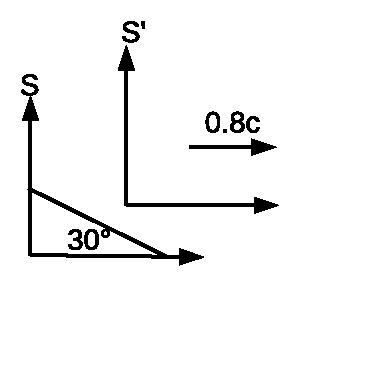
\includegraphics{fig1}

Note that,
\begin{align*}
	l_{ox} &= l_{o} \cos (30^{\circ}) = 1 \times \frac{\sqrt{3}}{2} =  \frac{\sqrt{3}}{2} \\
	l_{oy} &= l_{o} \sin (30^{\circ}) = 1 \times \frac{1}{2} =  \frac{1}{2}
\end{align*}
Now,
	Since the relative velocity of both the frames is perpendicular to the $y$-axis, the $y$-component of the length of the stick measures the same in both the frames. That is,
\begin{align*}
	l'_{oy} &= l_{oy} =  \frac{1}{2} \\
\end{align*}
Also, note that the $x$-xomponent of the rod can be thought of as "$proper$" in frame S (since the rod is at rest in the frame S). Hence, the $x$-component of the rod appears to be smaller than l$_{ox}$ ("$contracted$") by a factor of $\gamma$ when measured in S'. That is,
\begin{align*}
	l'_{ox} &= \frac{1}{\gamma} l_{ox}\\
	&=  \frac{1}{\frac{1}{\sqrt{1-\frac{(0.8c)^{2}}{c^{2}}}}} \times  l_{ox}\\
	&= \frac{3}{5} \times  l_{ox}\\
	&= \frac{3\sqrt{3}}{10}
\end{align*}
Hence, the length of the rod as seen in frame S' is given by
\begin{align*}
	{\bf l' = \sqrt{l'^{2}_{ox} + l'^{2}_{oy} } = \frac{\sqrt{13}}{5}}
\end{align*}
The orientation is similarly given.
\begin{align*}
	\theta ' &= \tan ^{-1}(\frac{l'_{oy}}{l'{_ox}}) \\
	&= {\bf 43.89^{\circ}}
\end{align*}

\item {\bf An observer A sees two events at the same place and separated in time by 1$\times$10$^{-6}$s. A second observer B sees them to be separated by 2$\times$10$^{-6}$s. What is the separation in space of the two events according to B? What is the speed of B with respect to A? } \\

{\underline {\bf Solution}} :

Note that, since the 2 events occur at the same place in A, the interval must be proper time in A.

Hence, $\Delta t_{B}$ = $\gamma \Delta t_{A}$.
Thus, $\gamma$ = 2\\
$\Rightarrow$ {\bf v = $\frac{\sqrt{3}}{2}$c}\\

Now, by Lorentz Transformation,
\begin{align*}
	\Delta x_{B} &= \gamma (\Delta x_{A} - v\Delta t_{A}) \\
	&= 2 (0 - \frac{\sqrt{3}}{2}c\times 1\times 10^{-6} ) \\
	&= {\bf -300\sqrt{3}  m}
\end{align*}


{\underline {\bf Alternate Solution}} :

Note that, since the 2 events occur at the same place in A, the interval must be proper time in A.

Hence, $\Delta t_{B}$ = $\gamma \Delta t_{A}$.
Thus, $\gamma$ = 2\\
$\Rightarrow$ {\bf v = $\frac{\sqrt{3}}{2}$c}\\

Also, the quantity
\begin{align*}
	\Delta \tau &= \sqrt{\Delta t^{2} - \frac{\Delta x^{2} + \Delta y^{2} + \Delta z^{2}}{c^{2}}}
\end{align*}
is an invariant and does not depend on the frame of reference. (Here, $\Delta \tau$ = 1$\times 10^{-6}$s )

For the frame of B, $\Delta t_{B}$ = 2$\times10^{-6}$s .
This means,
\begin{align*}
	\sqrt{\Delta x^{2}_{B} + \Delta y^{2}_{B} + \Delta z^{2}_{B}} &= {\bf 300\sqrt{3}  m}
\end{align*}

\end{enumerate}
\end{document} 
